\documentclass[tikz,border=10pt]{standalone}
\usepackage{amsmath}
\usetikzlibrary{arrows.meta, positioning, calc, decorations.pathreplacing}
\definecolor{c1}{HTML}{000000}
\definecolor{c2}{HTML}{233D4D}
\definecolor{c3}{HTML}{FE7F2D}
\definecolor{c4}{HTML}{EAECF0}
\definecolor{axiscolor}{HTML}{333333}
\definecolor{labelcolor}{HTML}{5F6B75}
\begin{document}
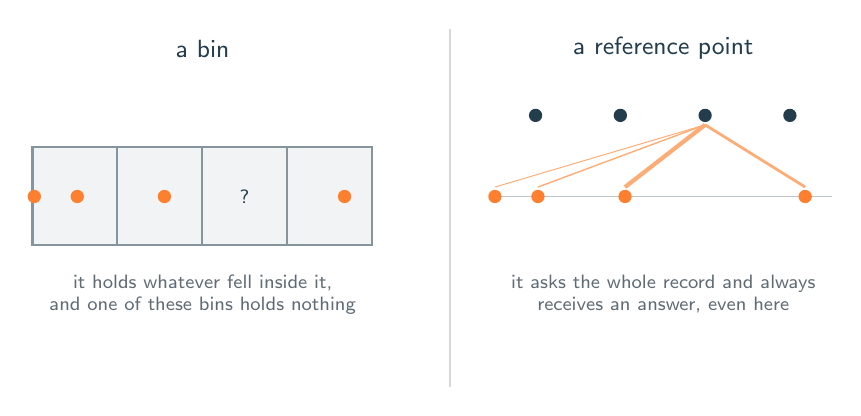
\begin{tikzpicture}[
    every node/.style={font=\sffamily},
    lab/.style={font=\sffamily\scriptsize, text=labelcolor},
    tag/.style={font=\sffamily\scriptsize, text=c2},
    hot/.style={font=\sffamily\scriptsize, text=c3!85!black},
]
\def\L#1{1.30 + #1*0.001500}
\def\R#1{7.15 + #1*0.001500}
\draw[c2!20, line width=0.8pt] (6.60, 0.50) -- (6.60, 5.05);
\node[tag, font=\sffamily\small] at (3.46, 4.80) {a bin};
\node[tag, font=\sffamily\small] at (9.31, 4.80) {a reference point};

% ---------------- left: bins
\foreach \b in {0,...,3}{
    \pgfmathsetmacro\a{\b*720}
    \pgfmathsetmacro\e{(\b+1)*720}
    \filldraw[draw=c2!55, fill=c2!6, line width=0.8pt]
        ({\L{\a}}, 2.30) rectangle ({\L{\e}}, 3.55);
}
\foreach \m/\v in {15/2.4, 380/3.1, 1120/4.6, 2650/2.8}{
    \fill[c3] ({\L{\m}}, 2.92) circle (2.4pt);
}
\node[tag] at ({\L{1800}}, 2.92) {?};
\node[lab, anchor=north, align=center] at (3.46, 2.05)
    {it holds whatever fell inside it,\\ and one of these bins holds nothing};

% ---------------- right: reference points
\draw[c2!30, line width=0.7pt] ({\R{0}}, 2.92) -- ({\R{2880}}, 2.92);
\foreach \m/\v in {15/2.4, 380/3.1, 1120/4.6, 2650/2.8}{
    \fill[c3] ({\R{\m}}, 2.92) circle (2.4pt);
}
\foreach \m in {360, 1080, 1800, 2520}{
    \fill[c2] ({\R{\m}}, 3.95) circle (2.4pt);
}
\foreach \m/\w in {15/0.35, 380/0.5, 1120/1.5, 2650/1.0}{
    \draw[c3!65, line width=\w pt] ({\R{1800}}, 3.83) -- ({\R{\m}}, 3.04);
}
\node[lab, anchor=north, align=center] at (9.31, 2.05)
    {it asks the whole record and always\\ receives an answer, even here};

\end{tikzpicture}
\end{document}
